\documentclass{article}

% preambulo:
\usepackage[utf8]{inputenc}
% caracteres utf8 (tildes, enie) sin tener que usar comandos

\usepackage[spanish, es-tabla, es-nodecimaldot]{babel} 
% texto automatico en espaniol
% "tabla" en vez de "cuadro"
% no reemplaza puntos decimales por comas

%% NO AGREGAR PAQUETES ANTES DE ESTO, ES IMPORTANTE QUE BABEL ESTE PRIMERO

%%%%%%%%%%%%%%%%%%%%%%%%%%%%%%%%%
%% PAQUETES EXTRA %%%%%%%%%%%%%%%
%%%%%%%%%%%%%%%%%%%%%%%%%%%%%%%%%

\usepackage{subfiles}

%nuevo
\usepackage[notransparent]{svg}
%

\usepackage{amsmath} % PAQUETES DE MATEMATICA
\usepackage{amsfonts}
\usepackage{amssymb}

%puse esta cosa nueva---
\usepackage{csvsimple}

%-----
\usepackage{steinmetz} % comando \phase{}
\usepackage{units} % permite usar nicefrac
\usepackage{graphicx} % importar imagenes
\usepackage{float} % posicion H para floats
\usepackage[colorinlistoftodos]{todonotes}


\usepackage[a4paper, total={6in, 8in}]{geometry} 
% margenes correctos en subarchivos

\setlength{\parindent}{10pt}			%cuanta sangria al principio de un parrafo
\usepackage{indentfirst}				%pone sangria al primer parrafo de una seccion

\usepackage{listings}

\usepackage{color}

\definecolor{codegreen}{rgb}{0,0.6,0}
\definecolor{codegray}{rgb}{0.5,0.5,0.5}
\definecolor{codepurple}{rgb}{0.58,0,0.82}
\definecolor{backcolour}{rgb}{0.95,0.95,0.92}
 
\lstdefinestyle{mystyle}{
    backgroundcolor=\color{backcolour},   
    commentstyle=\color{codegreen},
    keywordstyle=\color{magenta},
    numberstyle=\tiny\color{codegray},
    stringstyle=\color{codepurple},
    basicstyle=\footnotesize,
    breakatwhitespace=false,         
    breaklines=true,                 
    captionpos=b,                    
    keepspaces=true,                 
    numbers=left,                    
    numbersep=5pt,                  
    showspaces=false,                
    showstringspaces=false,
    showtabs=false,                  
    tabsize=2
}
 
\lstset{style=mystyle}

%%%%%%%%%%%%%%%%%%%%%%%%%%%%%%%%%%%%%%%%%%%%%%%%%%%%%%%%%%%
%% NO AGREGAR PAQUETES DESPUES DE ESTO, ES IMPORTANTE QUE HYPERREF ESTE ULTIMO
\usepackage[hidelinks]{hyperref} % hipervinculos sin cajitas rojas
\usepackage{bm}



\begin{document}

\newgeometry{} % margenes default para la caratula
% caratula:
\begin{titlepage}
\newcommand{\HRule}{\rule{\linewidth}{0.5mm}}
\center
\mbox{\textsc{\LARGE \bfseries {Instituto Tecnol\'ogico de Buenos Aires}}}\\[1.5cm]
\textsc{\Large 22.85 - Sistemas de Control}\\[0.5cm]


\HRule \\[0.6cm]
{ \Huge \bfseries Trabajo de Laboratorio N$^{\circ}$1: Phase-Locked Loop (PLL) o Lazo de Enganche de Fase}\\[0.4cm] % Title of your document
\HRule \\[1.5cm]


{\large

\emph{Grupo 1}\\
\vspace{3px}

\begin{tabular}{lr} 	
\textsc{M\'aspero}, Martina  & 57120 \\
\textsc{Mestanza}, Joaqu\'in Mat\'ias  & 58288 \\
\textsc{Nowik}, Ariel Santiago  & 58309 \\
\textsc{Panaggio Venerandi}, Guido Martin  & 56214 \\
\textsc{Parra}, Roc\'io  & 57669 \\
\textsc{Regueira}, Marcelo Daniel  & 58300 \\

\end{tabular}

\vspace{20px}

\emph{Profesor}\\
\vspace{3px}
\textsc{Nasini}, V\'ictor Gustavo\\ 	
\vspace{100px}

\begin{tabular}{ll}

Presentado: & 27/09/2019\\

\end{tabular}

}

\vfill

\end{titlepage}

% cambio los margenes para el resto del documento
\newgeometry{left=2.5cm, top=2.5cm, right=2cm, bottom=2cm}

% indice:
\tableofcontents
\newpage

\section*{Ejercicio 1: Prelaboratorio}
\addcontentsline{toc}{section}{Ejercicio 1: Prelaboratorio}
Se pidió analizar distintas transferencias (en la sección Prelaboratorio) del diagrama en bloques del circuito provisto por la cátedra.
\begin{figure}[H]
\centering
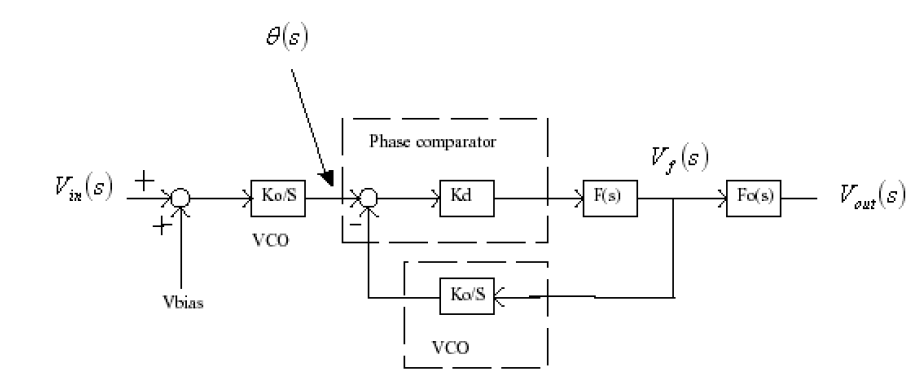
\includegraphics[width=1\linewidth]{images/Circuito.PNG}
\caption{Diagrama en bloques del circuito}
\label{fig:Circuito}
\end{figure}

\subsection*{a) Modulador (VCO)}

\begin{equation} \label{mod_eqn}
\frac{\theta(s)}{V_{in}(s)} = \frac{K_0}{s}
\end{equation}

\subsection*{b) Demodulador (PLL)}

\begin{equation} \label{demod_eqn}
\frac{V_f(s)}{\theta(s)} = \frac{s\cdot K_d \cdot F(s)}{s+K_0K_dF(s)}
\end{equation}

\subsection*{c) Filtros pasabajos: $F_1(s)$ y $F_2(s)$}
Como $F_1$ es $F_2$ con $R_6$ = 0, se analiza primero $F_2$.

\begin{equation} \label{f2_eqn}
F_2(s) = \frac{1+\frac{s}{\frac{1}{R_6 \cdot C_6}}}{ 1 + \frac{s}{\frac{1}{\left(R_5+R_6\right)\cdot C_6}}}
\end{equation}

\begin{equation} \label{f1_eqn}
F_1(s) = \frac{1}{ 1 + \frac{s}{\frac{1}{R_5\cdot C_6}}}
\end{equation}

\subsection*{d) $F_0(s)$}

\begin{equation} \label{fo_eqn}
F_0(s) = \frac{1}{ 1 + \frac{s}{\frac{1}{R_9\cdot C_7}}}
\end{equation}


\section*{Ejercicio 2: factor de amortiguamiento considerando los filtros}
\addcontentsline{toc}{section}{Ejercicio 2: factor de amortiguamiento considerando los filtros}


\begin{equation} \label{vftheta_eqn}
\frac{V_f(s)}{\theta(s)} = 
\frac{ 1 + \left(\frac{s}{\frac{1}{(\sqrt{C_6\cdot R_6}}}\right)^2 }
{ \left(\frac{s}{\omega_0}\right)^2 + 2\xi \omega_0 + 1}
\end{equation}

\begin{equation} \label{w0_eqn}
\omega_0 = \sqrt{\frac{K_d K_0}{C_6\cdot(R_5+R_6)}}
\end{equation}


\begin{equation} \label{xi_eqn}
\xi = \frac{(R_6 \cdot C_6\cdot K_d\cdot K_0  + 1) \sqrt{C_6 \cdot(R_5+R_6)}}
{2\cdot(K_d\cdot K_0)^\frac{3}{2}}
\end{equation}


\end{document}
